% !TEX encoding = UTF-8 Unicode
%%% Local Variables: 
%%% coding: utf-8
%%% mode: latex
%%% TeX-engine: xetex
%%% End: 

%\begin{figure}
%  \includegraphics[width=\linewidth]{boat.jpg}
%  \caption{A boat.}
%  \label{fig:boat1}
%\end{figure}

%Figure \ref{fig:boat1} shows a boat.

\documentclass[12pt]{article}
%\usepackage{fontspec}
%\setmainfont{Calibri}

\usepackage[utf8]{inputenc}
\usepackage[frenchb]{babel}
\usepackage{graphicx}
\usepackage{float}
\usepackage{url}

\usepackage[tmargin=2.54cm,bmargin=2.54cm,lmargin=3.19cm,rmargin=3.19cm]{geometry}

%\usepackage{frbib}

%\usepackage{apacite}
%\usepackage{bibentry}
%\usepackage[babel]{biblatex}

\renewcommand{\baselinestretch}{1.5} 

\setlength{\parskip}{12pt}

\usepackage{multirow}

\usepackage{adjustbox}

\usepackage{chngpage}

\begin{document}

% Bibliography Entries in Text
%
% In place of \bibliography{database}, enter \nobibliography{database}
% No bibliography is written at this point, but afterwards,
% \cite{key} prints the bibliography entry for citation <key>
% (whereas \cite{key} prints the citation, not the bib entry)
%
% If \bibliography is also to be given, then issue the starred variant
% \nobibliography* (without argument).

%
%
%	Titre
%
%


\title{Travail final}
\author{Laurent Tremblay,1642342}

%\pagestyle{fancy}

%
%Page d'introduction
%

%\pagenumbering{Roman}
\thispagestyle{empty}
\begin{center}

{\Large École Polytechnique de Montréal}


\vfill

{\Huge TP2 - Répartiteur de tâches\\}

\vfill

Benoît Paradis,  1677688\\
Laurent Tremblay,1642342 \\ 


\vfill

11 novembre 2016

\vfill

INF4410 \\ 
Systèmes répartis et infonuagique

\vfill

\includegraphics[scale=0.7]{Poly_Logo-eps-converted-to.pdf}

\end{center}
\newpage

%\section{Introduction}

\tableofcontents
\newpage

\bibliographystyle{apacite}
% \bibliography{mybib.bib}

\section{Introduction}

Une des idées principales d'un système répartis est d'être résilient, c'est à dire fortement tolérant aux pannes.
Il serait en effet impossible, pour n'importe quel système de taille non-triviale, de garantir le fonctionnement 
simultané de toute les machines le composant. Google a estimé, dans une étude publiée en 2007 \footnote{\url{https://static.googleusercontent.com/external_content/untrusted_dlcp/research.google.com/en//archive/disk_failures.pdf}}, que la probabilité qu'un disque dur 
brise pendant une année d'utilisation normale est de 1.7\% pour un disque neuf et de 8.6\% pour un disque de trois ans. 

%"actual annualized failure rates (AFRs) for individual drives ranged from 1.7% for first year drives to over 8.6% for three-year-old drives."
%https://static.googleusercontent.com/external_content/untrusted_dlcp/research.google.com/en//archive/disk_failures.pdf
%"Annualized failure rate (AFR) gives the estimated probability that a device or component will fail during a full year of use. 
%It is a relation between the mean time between failure (MTBF) and the hours that a number of devices are run per year. AFR is 
%estimated from a sample of like components—AFR and MTBF as given by vendors are population statistics that can not predict the 
%behaviour of an individual unit.[1]"

Ces valeurs, multipliées par la quantité de disques fonctionnant en même temps dans une infrastructure moderne, indique qu'un système doit
être capable de tolérer les pannes afin d'être utilisé de façon efficace. 

Le fait de répartir un système sur un ensemble de machines reliés entres-elles par un réseau implique aussi de devoir séparer un ensemble de tâches en 
sous-unités plus simples et de répartir ces tâches équitablement entre les nœuds du réseau afin d'obtenir une performance optimale. 

Notre répartiteur est un seul programme s'exécutant sur une machine et distribuant du travail à plusieurs nœuds de calculs.
C'est une architecture maître-esclave classique, tel qu'illustré à la figure \ref{fig:arch_1}.

\section{Présentation de l'architecture}

\begin{figure}
  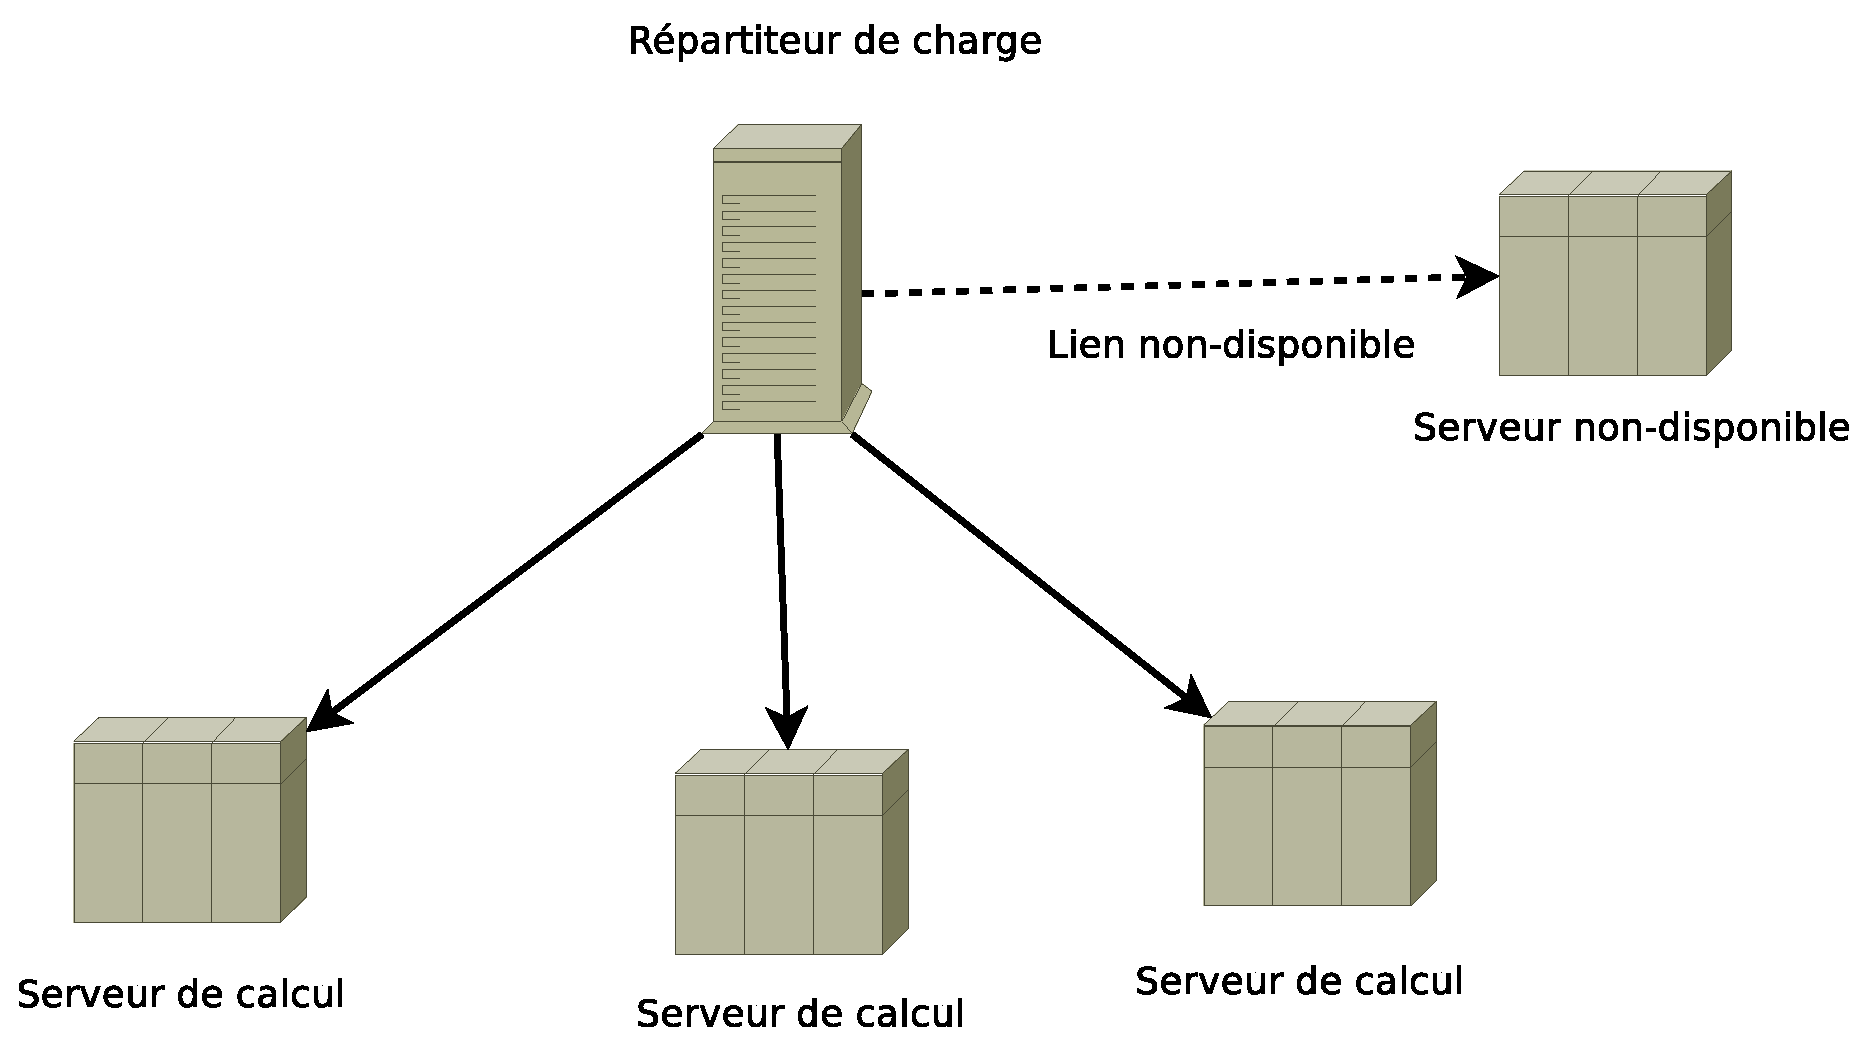
\includegraphics[width=\linewidth]{Arch_Trad.eps}
  \caption{L'architecture du répartiteur de charge}
  \label{fig:arch_1}
\end{figure}


Si le fait d'avoir plusieurs nœuds de calcul permet une redondance du système, le répartiteur en soi est un \emph{"singleton"} et 
ne comprend aucun mécanisme de redondance et représente un point unique de défaillance. Notre implémentation se doit d'être robuste et 
a donc été développé avec un style défensif. Certaines des \emph{"10 falacies of distributed computing"} ont été prise en compte lors de l'élaboration et implémentation
de notre architecture. 

Le serveur lui-même est écrit en utilisant un \emph{thread-pool} afin de gérer les serveurs de calcul. C'est une solution plus élégante et simple que 
d'attribuer un \emph{thread} par nœud de calcul, en raison du grand nombre potentiel de nœuds et du fait que les serveurs ne sont pas utilisés de façon intensive 
(on attribut un lot de travail et on attend de recevoir le résultat). 

Java RMI a été utilisé afin d'implémenter l'exécution de méthodes à distances. Ceci évite d'avoir à implémenter sois-même la couche réseau et permet
de profiter du mécanisme d'exceptions de Java ainsi que pouvoir isoler les erreurs de réseau lors du développement de l'application. L'utilisation 
de Java permet aussi de faire appel à des fonctions du langages, comme les \emph{Futures}, simplifiant grandement la réduction effectuée par le répartiteur. Celui-ci
attend en effet simplement que les \emph{Futures} soient disponibles. La communication entre les nœuds et le répartiteur est donc asynchrone par nature.  

L'implémentation non-sécuritaire repose sur un consensus où une majorité de machines doivent donner le même résultat pour une série d'opération données 
afin d'être considéré comme valide. 

%** TODO Déterminer le temps d'exécution des opérations 
%*** TODO Pel(0 -- 50)
%**** TODO fonction pour estimer 
%**** TODO graph
%*** TODO prime(0 -- MAX_INT)
%**** TODO fonction pour estimer 
%**** TODO graph
\subsection{Gestion des serveurs morts}
Puisque nous utilisons Java RMI pour exécuter les opérations sur les serveurs de calcul, il est possible d'utiliser les mécanismes d'exceptions de Java et 
de RMI afin de détecter si un serveur de calcul est indisponible. Le répartiteur recevra simplement une exception de type \emph{RemoteException}
quand il tentera d'exécuter un lot de travail sur un nœud n'étant plus disponible. Aucun mécanisme de \emph{keep-alive} n'est implémenté par le répartiteur, toute la communication 
entre le répartiteur et les nœuds étant encapsulé dans la couche de Java RMI. Le répartiteur peut ensuite donner le lot de travail à un autre nœud de calcul et périodiquement 
réessayer d'attribuer du travail au nœud ne répondant pas. Si la panne persiste, le répartiteur retirera simplement le nœud de calcul de sa liste de nœuds valides. La panne peut se
produire n'importe-quand durant l'exécution du lot de travail, puisque l'exécution d'un lot de travail est une opération atomique du point de vue du répartiteur (elle est soit exécutée au complet, 
refusée ou une exception est levée par Java RMI signalant qu'il est impossible de l'exécuter). 

%\subsection{Formation des "chunks de travail"}
%Puisque les opérations sont additionnés entres elles tout est commutatif, donc on peut 
%séparer le travail comme on veux. En utilisant les métriques de temps de calcul trouvés
%plus tôt, on peut créer des lots de travail de "valeurs" approximativement égales.
\subsection{Déterminer la capacité de chaque serveur }
Chaque serveur est vu comme une entité unique ayant des propriétés distinctes par le répartiteur. Le répartiteur ignorant le facteur q de chaque
serveur, ce dernier doit l'estimer. La stratégie pour estimer le facteur $ q $ est d'envoyer un lot de travail d'une taille donnée. Si ce dernier est accepté, on 
conserve la taille du lot de travail. Si ce dernier est refusé, on diminue la taille du lot de travail d'une opération et on tente de la re-soumettre. L'opération 
retirée est replacée dans la liste des opérations en attente et sera ajoutés à un prochain lot de travail. Une taille de 15 comme lot de travail initial a été 
choisie de façon empirique à partir des valeurs de q typiques données dans l'énoncé. Le fait de choisir un q légèrement plus gros que les valeurs de l'énoncé permet
de profiter du fait que certaines opérations où $ q > u $ pourraient quand-même être exécutées avant que, statistiquement, une d'entre-elles échoue et force le 
répartiteur à diminuer le nombre d'opérations dans sa requête. 

%\subsection{TODO Ajustement du répartiteur en fonction des serveurs }
%*** TODO Mesurer les performances de chaque lot par rapport au facteur heuristique calculé
%Le but est d'avoir aussi une approximation du facteur de qualité du réseau
%*** TODO Ajustement de la difficulté des items de travail. 
%Les noeuds ayant une moins grande capacité réelle se font attribuer des lots de travail plus 
%faciles, permettant d'avoir des lots plus équilibrés. 
\section{Test de performance - mode sécurisé}
L'exécution de \emph{operation-588} en mode sécuritaire donne les résultats présentés à la figure \ref{fig:safe}. Ces chiffres ont été obtenus en exécutant les serveurs et le client localement sur une machine. 

\begin{figure}
  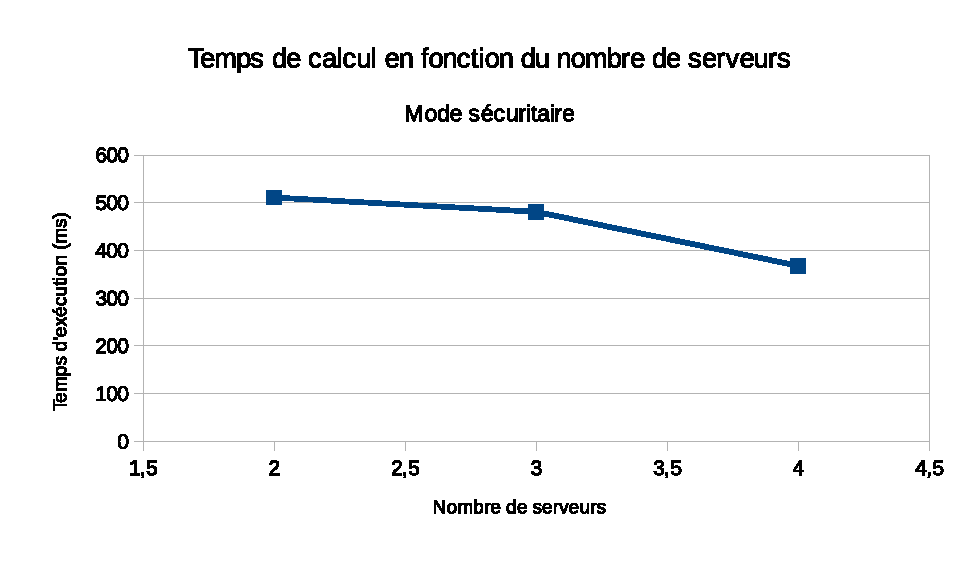
\includegraphics[width=\linewidth]{safe_exec.eps}
  \caption{ Exécution des différents tests de performance en mode sécuritaire }
  \label{fig:safe}
\end{figure}

On constate une amélioration de la performance lorsque plus de serveurs sont utilisés. Ceci s'explique par le fait que les
opérations sont fortement paralélisables. Puisque les tests ont été effectués sur une seule machine, il est impossible d'observer l'effet que le réseau aurait sur les résultats. On peut en revanche spéculer que dans l'environnemen du laboratoire, les performances seraient uniformément ralentie en raison de l'homogéniété du réseau local ainsi que de la petite taille des lots de travail et des appels de fonctions. 

\section{Test de performance - Mode non-sécurisé}

L'exécution de \emph{operation-588} en mode non-sécuritaire est plus lent que les résultats obtenus en utilisant les serveurs sécuritaires. Ceci est du à la nécéssité d'établir un consensus sur la valeur corecte des résultats avant de déclarer une opération comme complétée. L'algorithme de consensus consiste simplement à déclarer une valeur bonne si deux serveurs malicieux retourne la même valeur. Tant que deux serveurs n'auront pas retournés la même valeur, le répartiteur continuera d'attribuer le lot de travail correspondant à d'autre serveurs de calculs. Puisque un serveur malveillant envois une réponse aléatoire, il es peu probable que un serveur renvois deux fois la même réponse erroné. Ce cas extrèmenent rare causerait un re-calcul de l'ensemble des opérations puisque la somme de contrôle donnée avec chaque lot de travail ne corresponderait pas. Ce cas est extrèmenent lourd en terme de calculs mais se produira extrèmenent rarement, c'est pourquoi il a été décidé d'utiliser seulement un consensus à deux valeurs plutôt que 3, afin d'amortir le coût d'un recalcul complêt sur un très grand nombre d'opérations épargnées.

En faisant varier le pourcentage de réponses volotairement erronées des serveurs malveillants, on peut observer une dégradation de la performance causée par un plus grand nombre d'essais en moyenne avant d'obtenir deux résultats identiques. 

%3 serveurs de bonne foie, q = 5 : 755 ms

%2 serv de bonne foie, 1 50 % 951 ms

% 2 serv malicieux 50 %, un de bonne foie : 1108 ms

\section{Réponse Question 1}
Question 1: Le système distribué tel que présenté dans cet énoncé devrait être résilient aux pannes
des serveurs de calcul. Cependant, le répartiteur demeure un maillon faible. Présentez une
architecture qui permette d'améliorer la résilience du répartiteur. Quels sont les avantages et les
inconvénients de votre solution? Quels sont les scénarios qui causeraient quand même une panne du
système?

Notre approche serait de faire fonctionner plusieurs répartiteurs en parallèle, afin de permettre à 
un répartiteur de tomber en panne sans arrêter le système au complet. Dans un scénario idéal, les répartiteurs 
communiqueraient entre-eux afin de se distribuer un sous-ensemble des tâches à effectuer et confirmer aux autres répartiteurs 
les tâches ayant été données au nœuds de calculs et ayant été complétés, pour éviter qu'une même tâche ne soit exécuté deux fois
et comptabilisé deux fois. Ce n'est pas exceptionnellement grave si une tâche est exécuté deux fois, en autant que cette dernière ne sois 
pas comptabilisé deux fois lors de la réduction. Cette architecture est illustrée à la figure  \ref{fig:arch_2}.

\begin{figure}
  \includegraphics[width=\linewidth]{Arch_2.eps}
  \caption{Architecture éliminant le point unique de défaillance}
  \label{fig:arch_2}
\end{figure}

% - Problème du théorème CAP

% - "In theoretical computer science, the CAP theorem, also named Brewer's theorem after computer scientist Eric Brewer, states that it is impossible for a distributed computer system to simultaneously provide all three of the following guarantees:[1][2][3]

% Consistency (every read receives the most recent write or an error)
%Availability (every request receives a response, without guarantee that it contains the most recent version of the information)
%Partition tolerance (the system continues to operate despite arbitrary partitioning due to network failures)
%In other words, the CAP theorem states that in the presence of a network partition, one has to choose between consistency and availability."

Utiliser plusieurs répartiteurs indépendants pose toutefois un problème de taille : Une mauvaise configuration ou un problème 
de réseau peut maintenant partitonner notre infrastructure en deux, tel que les répartiteurs ne se "voient" plus, tel qu'illustré à la figure \ref{fig:arch_part}.

\begin{figure}
  \includegraphics[width=\linewidth]{Arch_2_part.eps}
  \caption{Partitionnement possible de l'architecture redondante}
  \label{fig:arch_part}
\end{figure}

On aurais le problème du P du théorème CAP, c'est à dire que le système peut devenir partitionnée et que les répartiteurs 
peuvent essayer d'assigner les mêmes tâches à deux serveurs sans se coordoner. Notre système doit donc faire le choix entre rester
disponible ou être consistant. 

Une solution serait de donner une copie de l'ensemble des tâches à réaliser à chaque répartiteur et d'utiliser des messages de synchronisation pour s'assurer que les 
tâches ne soient exécutées qu'une seule fois et comptabilisé une seule fois. Dans le cas d'un partitionnement, un seul des deux serveurs devrait continuer d'opérer normalement, 
un serveur dit "chef", l'autre se mettant en attente du premier serveur afin de se faire renvoyer la liste des tâches effectuées depuis le partitionnement par le serveur 
afin de pouvoir continuer l'exécution à deux serveurs en parallèle, tel qu'illustré à la figure \ref{fig:arch_2_chef}.

\begin{figure}
  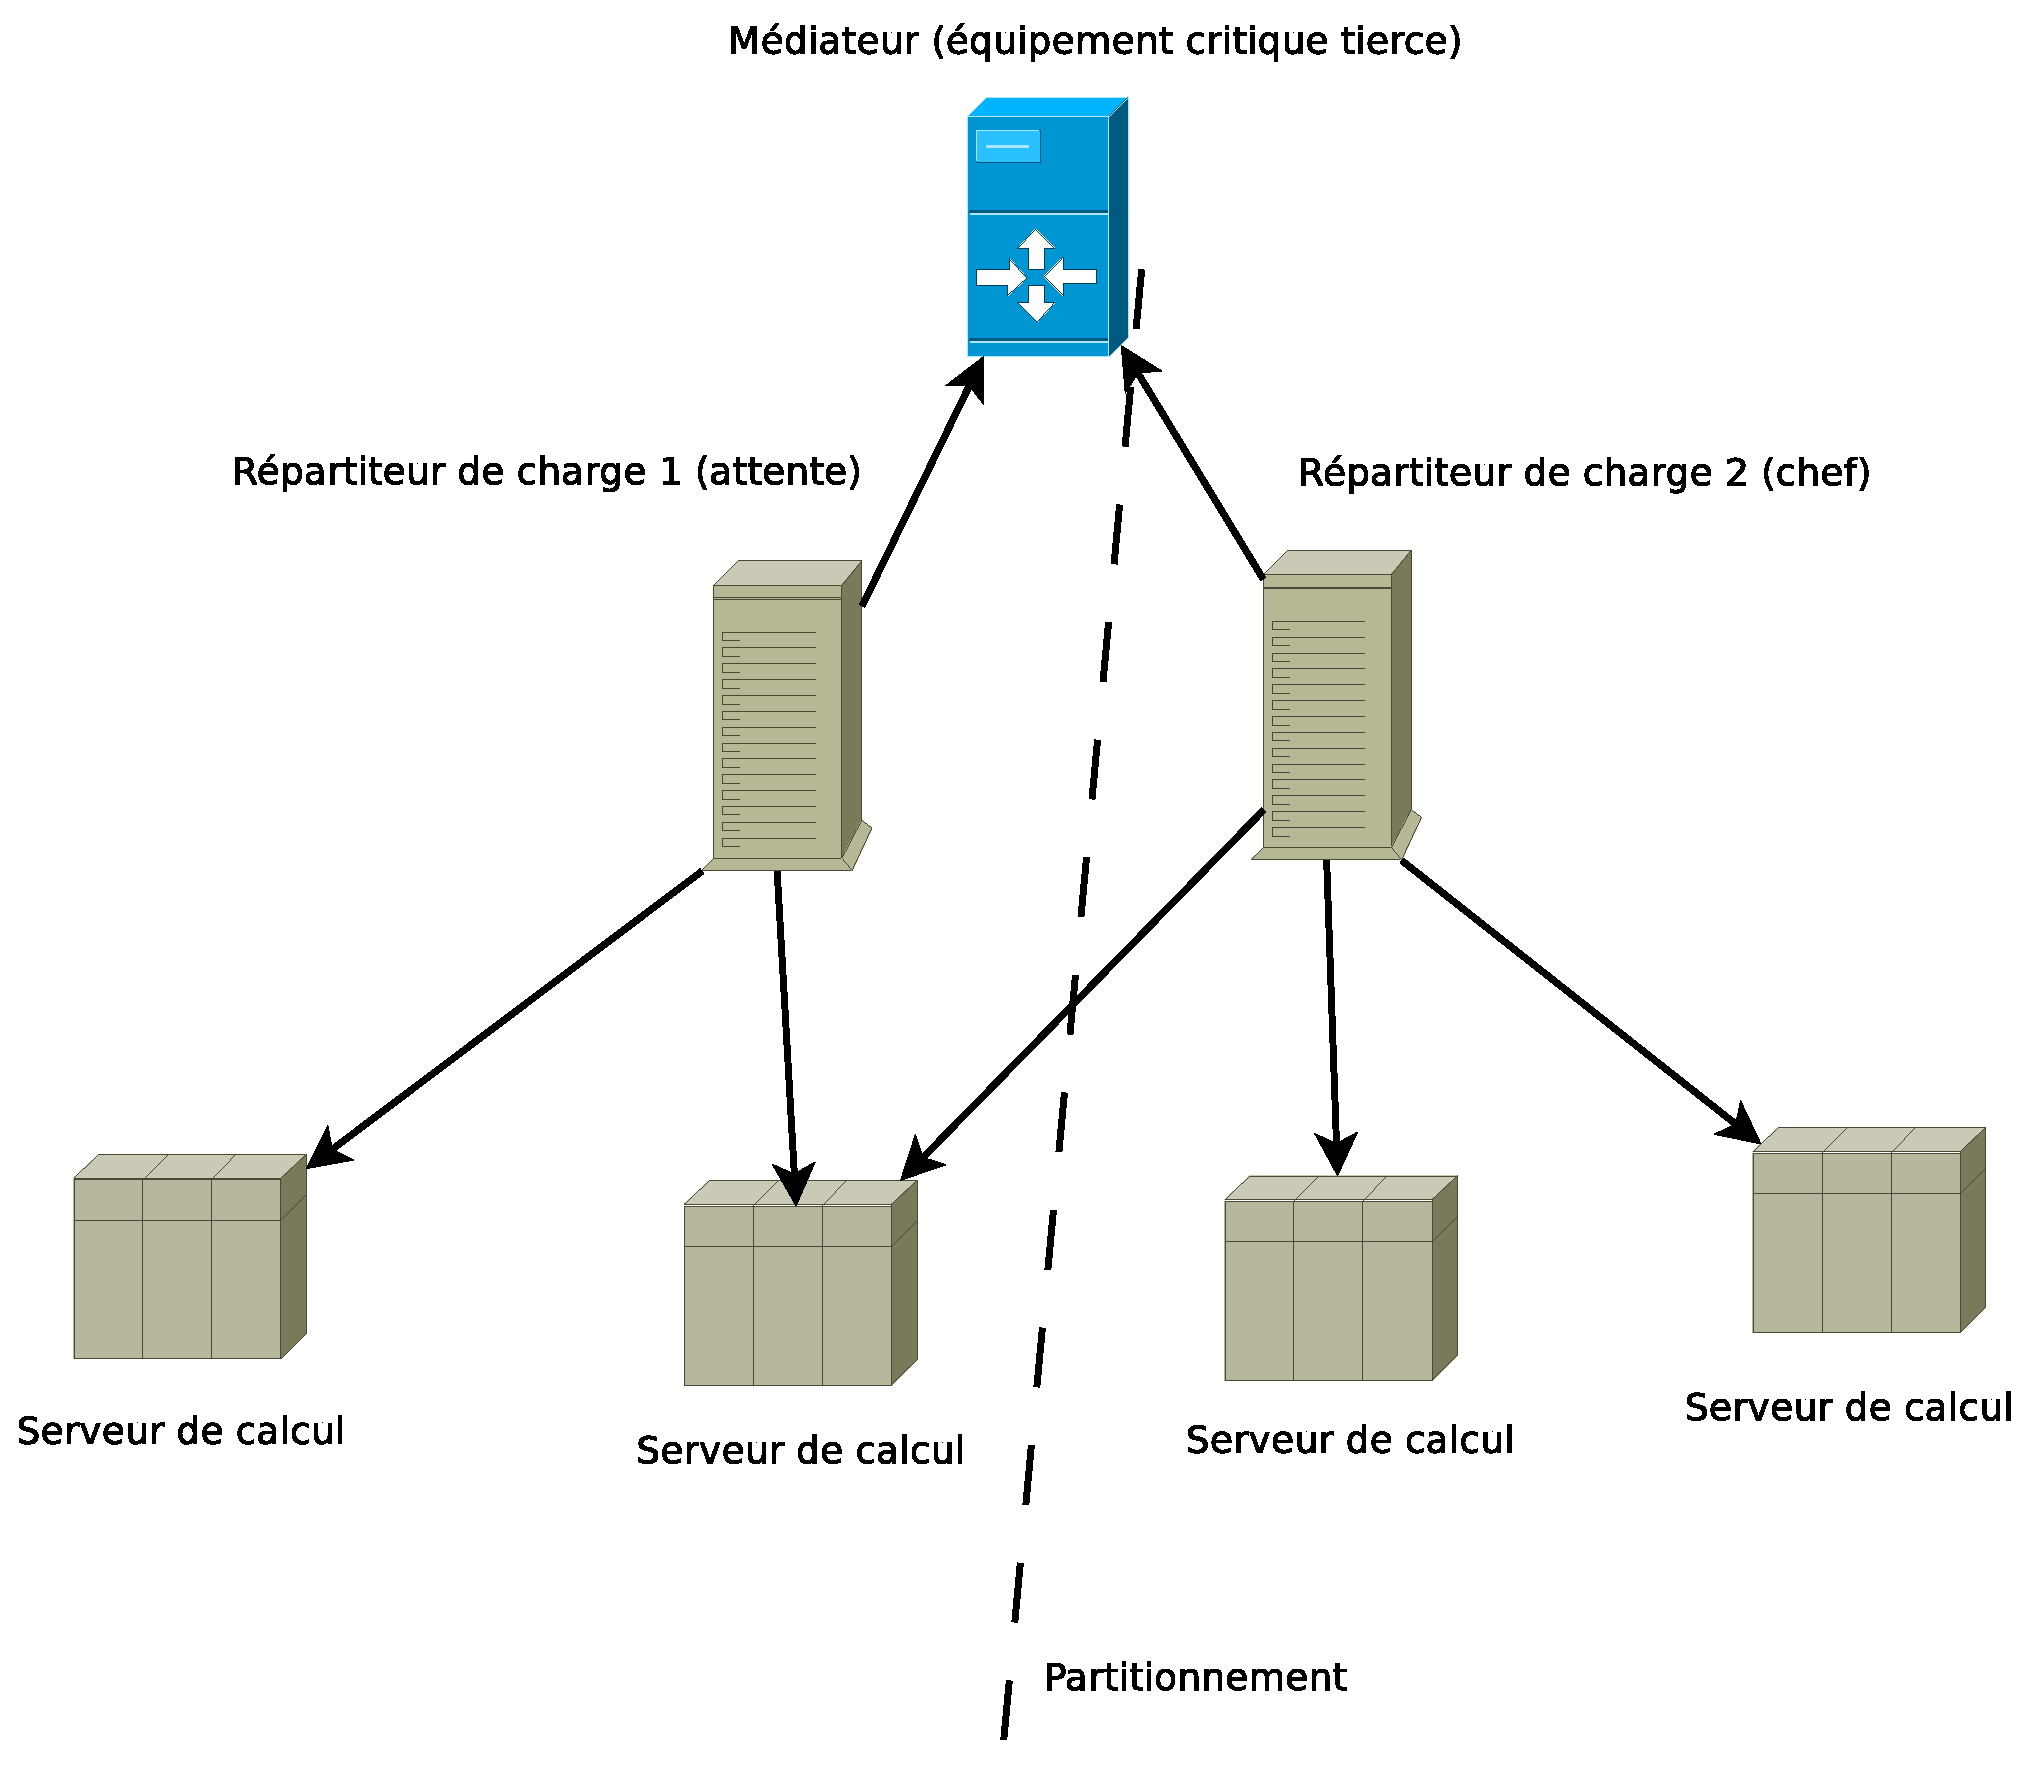
\includegraphics[width=\linewidth]{Arch_2_part_mediator.eps}
  \caption{Médiation du partitionnement par un arbitre externe}
  \label{fig:arch_2_chef}
\end{figure}

Cette approche permet une consistance des données (on retombe dans le cas du maître-esclave traditionnel
et du singleton) mais le système sera plus lent et moins disponible. 

Un problème de cette approche est toutefois d'identifier le partitionnement lorsque ce dernier se produit et de déterminer quel répartiteur doit agir comme "chef". Le cas trivial d'un 
serveur totalement déconnecté du réseau est évident à traiter, puisque ce dernier ne peut plus voir aucun autre nœud ou répartiteur, mais le cas où la partition isole les répartiteurs 
l'un de l'autre mais où des nœuds de calculs sont toujours accessibles, déterminer un chef est un problème de taille en sois. Une solution serait de choisir une machine tierce comme point de 
référence pour notre système, comme une \emph{switch} réseau centrale où un serveur particulièrement robuste. En cas de partitionnement, tout serveur étant capable de rejoindre cette pièce d'équipement 
sera le répartiteur "chef". Cette solution permet même à cette pièce d'équipement, de signaler qu'elle a déjà donné le contrôle à un autre répartiteur, si deux répartiteurs sont capable de la contacter. 
Cette solution est toutefois vulnérable à d'autres scénarios de partitionnement. 

Une autre approche est de faire travailler les répartiteurs comme si de rien était mais sans effectuer la réduction finale sur les résultats des calculs. Quand un autre répartiteur reviendra accessible, 
ces derniers communiqueront quelles opérations ils ont effectués et s'assureront d'effectuer la réduction uniquement une fois sur chaque opération. 

Une dernière approche serait de donner des états aux serveurs de calcul, mais cette approche comporte aussi son lot de problèmes additionnels. 
Nous préférons grandement une implémentation où les serveurs de calculs agissent sans conserver d'états, comme dans une architecture REST traditionnelle. 

\section{Conclusion et implémentations alternatives.}

En terme d'optimisations, notre répartiteur repose sur plusieurs heuristiques (choix du nombre de requêtes initial) n'ayant pas été étudiés. 
Un profilage détaillé de l'application ainsi que la variation de ces paramètres pourrait permettre de les fixer à des valeurs optimales en fonction
du type de charge de travail à effectuer. De plus, notre implémentation se base sur un réseau relativement fiable et constant en terme de latence et de débit. 
Aucune optimisation n'est effectués pour se protéger d'un réseau fiable mais au performances aléatoires. À titre d'exemple, le choix des serveurs ne se fait pas 
en prenant en compte la performance du réseau. Un serveur inoccupé mais connecté à un réseau très lent sera favorisé par rapport à un serveur très occupé mais connecté
à un réseau très rapide et offrant, au final, de meilleures performances. Une façon de remédier à ce problème serait de faire mesurer le temps de réponse d'un serveur
pour une requête donnée par le répartiteur et la comparer à une valeur heuristique correspondant à l'exécution locale de ce lot de travail afin de déterminer la
pénalité imposé par le réseau pour utiliser ce nœud en particulier. 

Il serait aussi possible d'obtenir le facteur d'utilisation des serveurs directement en les interrogeant plutôt qu'en envoyant des lots de travail de taille 
aléatoire. Théoriquement, rien n'empêche le serveur de renvoyer des informations sur sa charge de travail actuelle.

Il aurait été possible de tenter d'estimer l'honnêteté d'un serveur non-sécuritaire afin d'envoyer plus de requêtes aux serveurs donnant les bons résultat la majorité du temps. 

Finalement, il serait aussi possible de mieux équilibrer la charge de travail entre différents lots de même taille.Puisque le temps de calcul du plus grand nombre premier crois linéairement avec la valeur du nombre à traiter, un lot de travail comportant uniquement des nombres de très grande valeur sera plus long à exécuter qu'un lot de même taille comportant des valeurs très petites. Pour équilibrer les lots, il faudrait mesurer la performance des opérations afin d'assigner une valeur estimée de difficulté pour une opération donnée et tenter de former les lots de travail de façon à ce que la somme des difficultés soit relativement uniforme d'un lot à l'autre. 


\end{document}

%
%
%  Fin du document
%
%
%
%
